\begin{figure}[!htb]
    \centering
    \caption{\textbf{Impact of Noise on Mean Wealth Distribution (Standardize)} \\ 
    \small{
    The figure shows the distribution of the estimated parameters when we add a random number from a normal distribution with mean 0 and standard deviation 0.1 to the mean wealth. We re-estimate the model using the new moments for 1000 times and compare the results with the original estimates.  We normalize the results by dividing them by the standard deviation of the results and subtracting the mean of the results.
    The blue line represents the estimates for different values of the mean wealth. The dashed lines represent the 5th and 95th percentiles of the distribution of the estimated parameters.
    We report the results for $\beta$ in (a), $\gamma$ in (b), and $\phi$ in (c).
    }
    }
    \label{fig:robustness_standard_check}

    \subfloat[][Robustness Check for $\beta$]{
    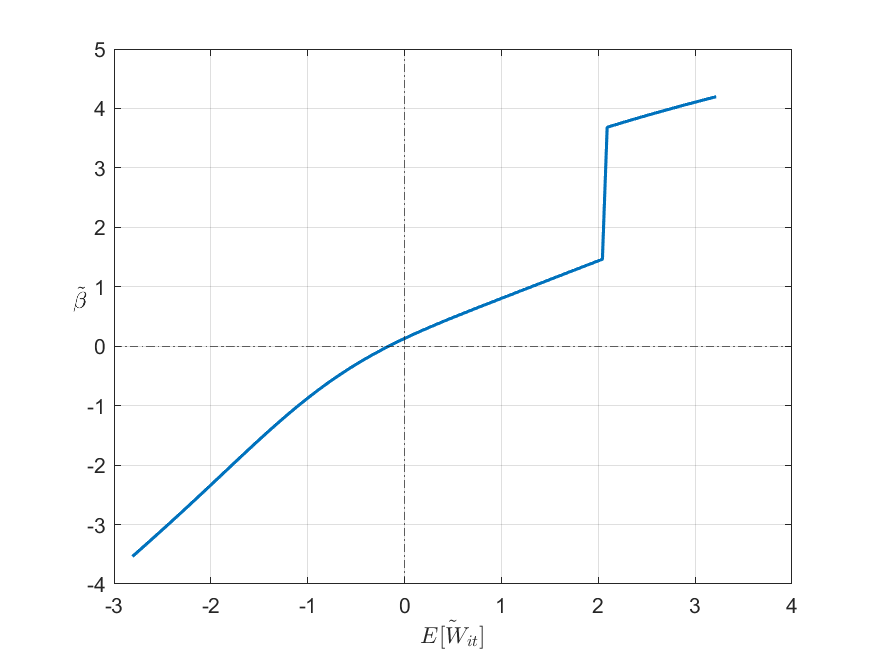
\includegraphics[width=0.45\linewidth]{Figures/robustness_check_parameter_normalize_beta.png}
    }   
    \subfloat[][Robustness Check for $\gamma$]{
    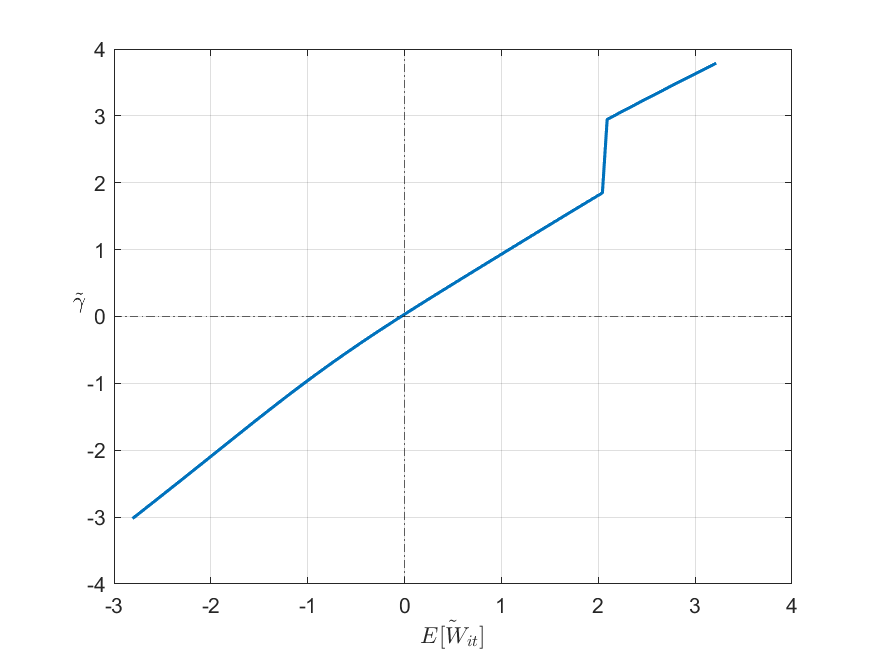
\includegraphics[width=0.45\linewidth]{Figures/robustness_check_parameter_normalize_gamma.png}
    }\\
    \subfloat[][Robustness Check for $\phi$]{
    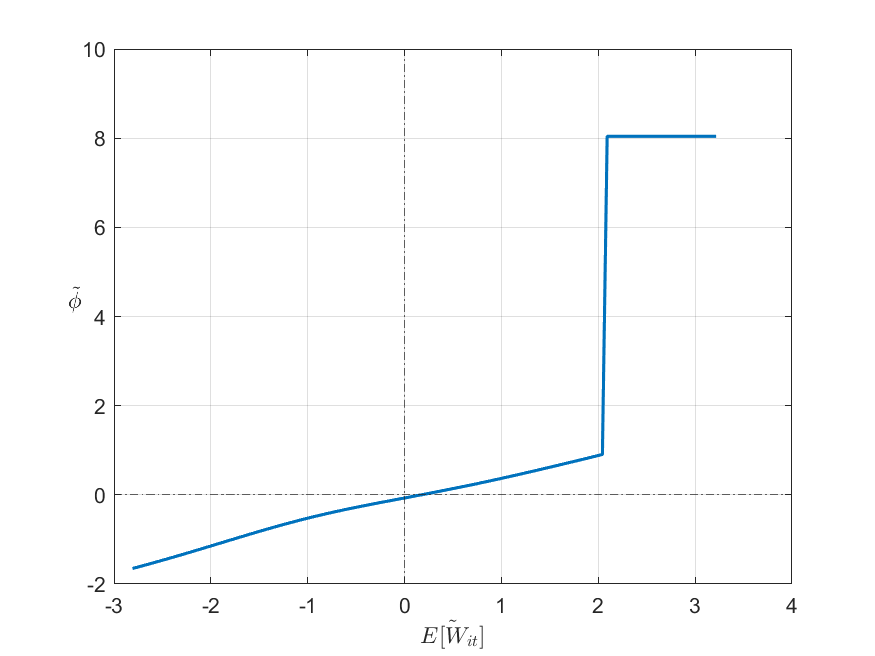
\includegraphics[width=0.45\linewidth]{Figures/robustness_check_parameter_normalize_phi.png}
    }
\end{figure}